\documentclass[tikz,border=6pt]{standalone}
\usepackage{helvet}
\usetikzlibrary{arrows.meta}
\definecolor{kspace}{HTML}{DAE8FC}
\definecolor{kborder}{HTML}{7C9AC4}
\definecolor{library}{HTML}{D5E8D4}
\definecolor{lborder}{HTML}{82B366}
\definecolor{data}{HTML}{009900}
\definecolor{dataarrow}{HTML}{9ACA7F}
\definecolor{energy}{HTML}{F8CECC}
\definecolor{eborder}{HTML}{B85450}
\begin{document}
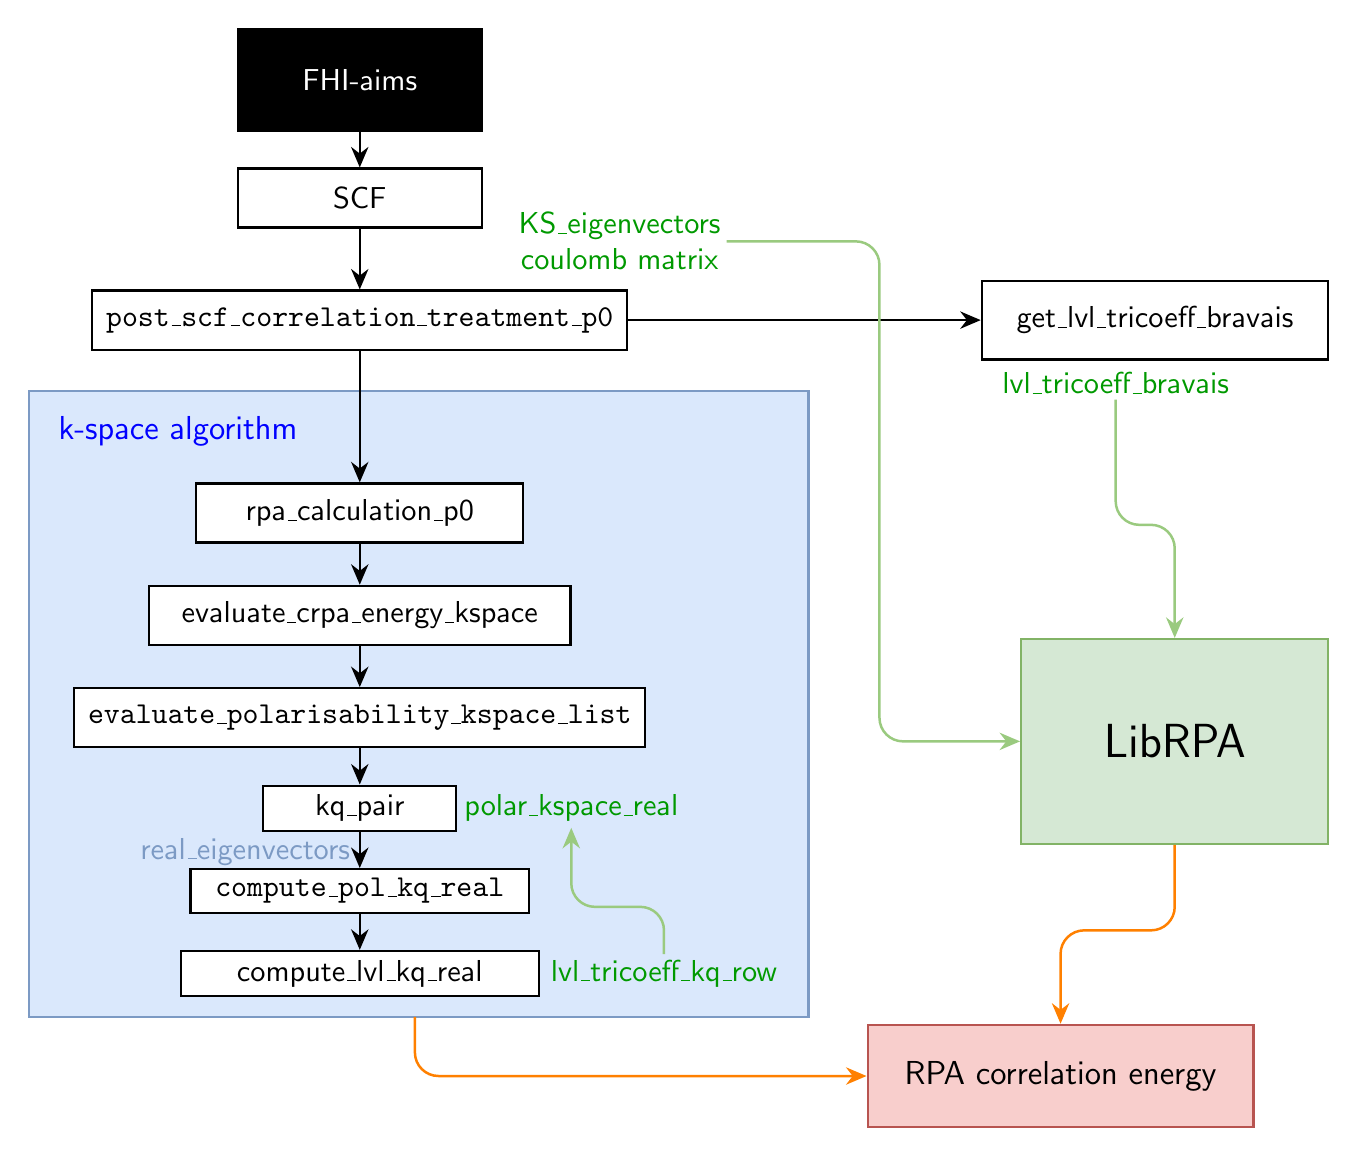
\begin{tikzpicture}[
  font=\sffamily\fontsize{11}{13}\selectfont,
  box/.style={draw=black,line width=.8pt,fill=white,align=center,
    minimum height=.75cm,inner xsep=5pt},
  arrow/.style={-{Stealth[length=2.6mm,width=2.2mm]},line width=.9pt},
  datalabel/.style={text=data,align=center,inner sep=2pt}]

\draw[fill=kspace,draw=kborder,line width=1pt]
  (.2,1.6) rectangle (10.1,9.55);
\node[anchor=north west,text=blue,font=\sffamily\fontsize{13}{16}\selectfont]
  at (.45,9.35) {k-space algorithm};

\node[box,fill=black,text=white,minimum width=3.1cm,minimum height=1.3cm]
  (aims) at (4.4,13.5) {FHI-aims};
\node[box,minimum width=3.1cm] (scf) at (4.4,12.0) {SCF};
\node[box,font=\ttfamily\fontsize{11}{13}\selectfont] (post) at (4.4,10.45)
  {post\_scf\_correlation\_treatment\_p0};
\node[box,minimum width=4.15cm] (rpa) at (4.4,8.0)
  {rpa\_calculation\_p0};
\node[box,minimum width=5.35cm] (energy) at (4.4,6.7)
  {evaluate\_crpa\_energy\_kspace};
\node[box,font=\ttfamily\fontsize{11}{13}\selectfont] (polar) at (4.4,5.4)
  {evaluate\_polarisability\_kspace\_list};
\node[box,minimum width=2.45cm,minimum height=.5cm] (pair) at (4.4,4.25)
  {kq\_pair};
\node[box,minimum width=4.3cm,minimum height=.5cm,font=\ttfamily\fontsize{11}{13}\selectfont]
  (pol) at (4.4,3.2) {compute\_pol\_kq\_real};
\node[box,minimum width=4.55cm,minimum height=.5cm] (lvl) at (4.4,2.15)
  {compute\_lvl\_kq\_real};
\draw[arrow] (aims) -- (scf);
\draw[arrow] (scf) -- (post);
\draw[arrow] (post) -- (rpa);
\draw[arrow] (rpa) -- (energy);
\draw[arrow] (energy) -- (polar);
\draw[arrow] (polar) -- (pair);
\draw[arrow] (pair) -- (pol);
\draw[arrow] (pol) -- (lvl);

\node[text=kborder,anchor=east] at (4.4,3.7) {real\_eigenvectors};
\node[datalabel,anchor=west] (pk) at (5.65,4.25) {polar\_kspace\_real};
\node[datalabel,anchor=west] (ck) at (6.75,2.15) {lvl\_tricoeff\_kq\_row};
\draw[arrow,dataarrow,rounded corners=3mm]
  (ck.north) -- ++(0,.6) -| (pk.south);

\node[box,minimum width=4.4cm,minimum height=1cm] (bravais) at (14.5,10.45)
  {get\_lvl\_tricoeff\_bravais};
\draw[arrow] (post) -- (bravais);
\node[datalabel] (cr) at (14.0,9.65) {lvl\_tricoeff\_bravais};
\node[box,fill=library,draw=lborder,minimum width=3.9cm,
  minimum height=2.6cm,font=\sffamily\LARGE] (librpa) at (14.75,5.1) {LibRPA};
\draw[arrow,dataarrow,rounded corners=3mm]
  (cr.south) -- (14,7.85) -- (14.75,7.85) -- (librpa.north);
\node[datalabel] (ks) at (7.7,11.45) {KS\_eigenvectors\\coulomb matrix};
\draw[arrow,dataarrow,rounded corners=3mm]
  (ks.east) -- (11.0,11.45) -- (11.0,5.1) -- (librpa.west);

\node[box,fill=energy,draw=eborder,minimum width=4.9cm,
  minimum height=1.3cm,font=\sffamily\large] (out) at (13.3,.85)
  {RPA correlation energy};
\draw[arrow,orange,rounded corners=3mm]
  (librpa.south) -- (14.75,2.7) -- (13.3,2.7) -- (out.north);
\draw[arrow,orange,rounded corners=3mm]
  (5.1,1.6) -- (5.1,.85) -- (out.west);
\end{tikzpicture}
\end{document}
